
%%--------------------------------------------------
%% CPO: Multiple Choice Questions
%%--------------------------------------------------


%% Chapter 23: Optics
%%--------------------------------------------------


%% Learning Objectives
%%--------------------------------------------------

%% Describe how simple optical devices work. 
%% Explain the difference between converging and diverging lenses. 
%% Understand how light is affected by matter. 
%% Explain the law of reflection. 
%% Describe what happens when light goes from one material to another. 
%% Understand the index of refraction.
%% Learn about total internal reflection and optics. 
%% Explain why different colors of light refract differently. 
%% Explain how images are formed. 
%% Explain the difference between a real and a virtual image.
%% Describe how to draw a ray diagram.


%% CPO Multiple Choice Questions
%%--------------------------------------------------
\element{cpo-mc}{
\begin{question}{cpo-ch23-q01}
    A glass window is best described as a(n) \rule[-0.1pt]{4em}{0.1pt} material.
    \begin{multicols}{2}
    \begin{choices}
      \correctchoice{transparent}
        \wrongchoice{translucent}
        \wrongchoice{absorbing}
        \wrongchoice{reflecting}
    \end{choices}
    \end{multicols}
\end{question}
}

\element{cpo-mc}{
\begin{question}{cpo-ch23-q02}
    Wax paper is best described as a(n) \rule[-0.1pt]{4em}{0.1pt} material.
    \begin{multicols}{2}
    \begin{choices}
        %% NOTE: corrected exam book
        \wrongchoice{transparent}
      \correctchoice{translucent.}
        \wrongchoice{absorbing.}
        \wrongchoice{reflecting.}
    \end{choices}
    \end{multicols}
\end{question}
}

\element{cpo-mc}{
\begin{question}{cpo-ch23-q03}
    A black asphalt road is best described as a(n) \rule[-0.1pt]{4em}{0.1pt} material.
    \begin{multicols}{2}
    \begin{choices}
        %% NOTE: corrected exam book again
        \wrongchoice{transparent}
        \wrongchoice{translucent.}
      \correctchoice{absorbing.}
        \wrongchoice{reflecting.}
    \end{choices}
    \end{multicols}
\end{question}
}

\element{cpo-mc}{
\begin{question}{cpo-ch23-q04}
    A converging lens \emph{always}:
    \begin{choices}
      \correctchoice{causes light rays to come together.}
        \wrongchoice{makes objects viewed through them appear smaller.}
        \wrongchoice{causes light rays to spread apart.}
        \wrongchoice{distorts light by reflecting it in different directions.}
    \end{choices}
\end{question}
}

\element{cpo-mc}{
\begin{question}{cpo-ch23-q05}
    The light ray which strikes the surface of an optical device is known as the \rule[-0.1pt]{4em}{0.1pt} ray.
    \begin{multicols}{2}
    \begin{choices}
      \correctchoice{incident}
        \wrongchoice{reflected}
        \wrongchoice{refracted}
        \wrongchoice{diffuse}
    \end{choices}
    \end{multicols}
\end{question}
}

\element{cpo-mc}{
\begin{question}{cpo-ch23-q06}
    The type of reflection in which the light is scattered into many directions is known as:
    \begin{multicols}{2}
    \begin{choices}
        \wrongchoice{specular.}
        %% NOTE: also lambertian
      \correctchoice{diffuse.}
        \wrongchoice{refracted.}
        \wrongchoice{regular.}
    \end{choices}
    \end{multicols}
\end{question}
}

\element{cpo-mc}{
\begin{question}{cpo-ch23-q07}
    All of the following statements about perfectly polished surfaces are true \emph{except}:
    \begin{choices}
        \wrongchoice{the surface itself seems invisible.}
      \correctchoice{the surface creates diffuse reflection.}
        \wrongchoice{all parallel light rays from a source are reflected parallel by the surface.}
        \wrongchoice{the surface creates specular reflections.}
    \end{choices}
\end{question}
}

\element{cpo-mc}{
\begin{question}{cpo-ch23-q08}
    Simply optical devices include lenses, mirrors, and:
    \begin{multicols}{2}
    \begin{choices}
        \wrongchoice{pencils.}
        \wrongchoice{pens.}
      \correctchoice{prisms.}
        \wrongchoice{crayons.}
    \end{choices}
    \end{multicols}
\end{question}
}

\element{cpo-mc}{
\begin{question}{cpo-ch23-q09}
    The diagram below represents a light ray striking a flat mirror.
    \begin{center}
    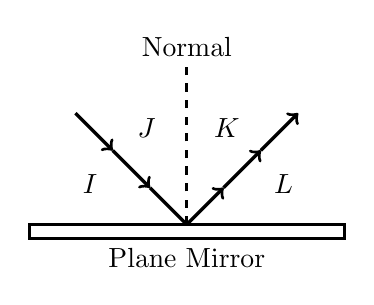
\begin{tikzpicture}
        \draw[very thick] (-2,0) rectangle (2,-0.5em);
        \node[anchor=north] at (0,-0.5em) {Plane Mirror};
        \draw[very thick,dashed] (0,0) -- (0,2)
            node[anchor=south] {Normal};
        \draw[very thick,->] (135:2.00) -- (135:1.33);
        \draw[very thick,->] (135:1.33) -- (135:0.66);
        %% NOTE: Change where arrow heads are
        \draw[very thick] (135:0.66) -- (135:0.00);
        \draw[very thick,->] (45:0.00) -- (45:0.66);
        \draw[very thick,->] (45:0.66) -- (45:1.33);
        \draw[very thick,->] (45:1.33) -- (45:2.00);
        \node[anchor=center] at (22.5:1.33) {$L$};
        \node[anchor=center] at (67.5:1.33) {$K$};
        \node[anchor=center] at (112.5:1.33) {$J$};
        \node[anchor=center] at (157.5:1.33) {$I$};
    \end{tikzpicture}
    \end{center}
    Which angle represents the angle of reflection?
    \begin{multicols}{4}
    \begin{choices}
        \wrongchoice{$I$}
        \wrongchoice{$J$}
      \correctchoice{$K$}
        \wrongchoice{$L$}
    \end{choices}
    \end{multicols}
\end{question}
}

\element{cpo-mc}{
\begin{question}{cpo-ch23-q10}
    The line drawn on a ray diagram perpendicular to the surface at the point where the incoming light strikes the surface is called the:
    \begin{multicols}{2}
    \begin{choices}
        \wrongchoice{ray}
      \correctchoice{normal line}
        \wrongchoice{incident light}
        \wrongchoice{reflected light}
    \end{choices}
    \end{multicols}
\end{question}
}

\element{cpo-mc}{
\begin{question}{cpo-ch23-q11}
    All of the following statements correctly describe light rays \emph{except} that light rays:
    \begin{choices}
      \correctchoice{can be seen coming from a light by squinting your eyes.}
        \wrongchoice{can be used to predict the size and location of an image.}
        \wrongchoice{are often represented with arrows on ray diagrams.}
        \wrongchoice{are imaginary lines with represent a thin beam of light.}
    \end{choices}
\end{question}
}

\element{cpo-mc}{
\begin{question}{cpo-ch23-q12}
    You can clearly see yourself in a flat (plan) mirror because of which kind of reflection?
    \begin{multicols}{2}
    \begin{choices}
        \wrongchoice{Real}
      \correctchoice{Specular}
        %% NOTE: also lambertian
        \wrongchoice{Diffuse}
        \wrongchoice{Refracted}
    \end{choices}
    \end{multicols}
\end{question}
}

\element{cpo-mc}{
\begin{question}{cpo-ch23-q13}
    The diagram below represents a light ray striking a flat mirror.
    \begin{center}
    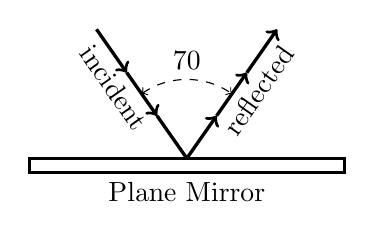
\begin{tikzpicture}
        \draw[very thick] (-2,0) rectangle (2,-0.5em);
        \node[anchor=north] at (0,-0.5em) {Plane Mirror};
        \draw[very thick,->] (125:2.00) -- (125:1.33);
        \draw[very thick,->] (125:1.33) -- (125:0.66);
        %% NOTE: Change where arrow heads are
        \draw[very thick] (125:0.66) -- (125:0.00);
        \node[anchor=north west,rotate=-55] at (125:2) {incident};
        \draw[very thick,->] (55:0.00) -- (55:0.66);
        \draw[very thick,->] (55:0.66) -- (55:1.33);
        \draw[very thick,->] (55:1.33) -- (55:2.00);
        \node[anchor=north east,rotate=55] at (55:2) {reflected};
        \draw[<->,dashed] (125:1.00) arc (125:55:1.00)
            node[pos=0.5,anchor=south] {\ang{70}};
    \end{tikzpicture}
    \end{center}
    What is the value in degrees for the angle of incidence?    
    \begin{multicols}{2}
    \begin{choices}
        \wrongchoice{\ang{20}}
      \correctchoice{\ang{35}}
        \wrongchoice{\ang{55}}
        \wrongchoice{\ang{70}}
    \end{choices}
    \end{multicols}
\end{question}
}

\element{cpo-mc}{
\begin{question}{cpo-ch23-q14}
    According to the law of reflection, the angle of incidence is always:
    \begin{choices}
        \wrongchoice{bigger than the angle of reflection.}
      \correctchoice{equal to the angle of reflection.}
        \wrongchoice{smaller than the angle of reflection.}
        \wrongchoice{determined by measuring between the incident and reflected rays.}
    \end{choices}
\end{question}
}

\element{cpo-mc}{
\begin{question}{cpo-ch23-q15}
    You are holding a paper with the word \emph{PHYSICS} printed on it in front of a flat mirror.
    All of the following statements about the image formed by the mirror are correct \emph{except} that the:
    \begin{choices}
        \wrongchoice{image appears twice as far from you as you are from the mirror.}
        \wrongchoice{image is the same size as you.}
        \wrongchoice{word \emph{PHYSICS} is written backward in the mirror.}
      \correctchoice{word \emph{PHYSICS} is written upside down the mirror.}
    \end{choices}
\end{question}
}

%\element{cpo-mc}{
%\begin{question}{cpo-ch23-q16}
%    An object is placed in front of a mirror as shown in the
%        diagram below.
%    \begin{center}
%        %% NOTE: add diagram
%    \end{center}
%    Which diagram represents the image of that object in the mirror?
%    \begin{choices}
%        \wrongchoice{
%            \begin{tikzpicutre}
%            \end{tikzpicture}
%        }
%    \end{choices}
%\end{question}
%}

%\element{cpo-mc}{
%\begin{question}{cpo-ch23-q17}
%    A tall person's eye level is at \SI{2.0}{\meter} high and his
%        feet are at \SI{0.0}{\meter} high:
%    \begin{center}
%        %% NOTE: add diagram
%    \end{center}
%    If light rays are reflected so that he is able to see an
%        image of his feet, approximately how far from the floor
%        do these rays strike the mirror?
%    \begin{multicols}{2}
%    \begin{choices}
%        \wrongchoice{\SI{2.0}{\meter}.}
%      \correctchoice{\SI{1.0}{\meter}.}
%        \wrongchoice{\SI{0.25}{\meter}.}
%        \wrongchoice{\SI{0.0}{\meter}.}
%    \end{choices}
%    \endn{multicols}
%\end{question}
%}

\element{cpo-mc}{
\begin{question}{cpo-ch23-q18}
    The bending of a light ray as it travels from air into water is known as:
    \begin{multicols}{2}
    \begin{choices}
        \wrongchoice{specularization}
        \wrongchoice{reflection}
      \correctchoice{refraction}
        \wrongchoice{diffusion}
    \end{choices}
    \end{multicols}
\end{question}
}

\element{cpo-mc}{
\begin{question}{cpo-ch23-q19}
    When light passes, as shown in the illustration below,
         from a material with a smaller index of refraction into a material with a higher index of refraction it will:
    \begin{center}
    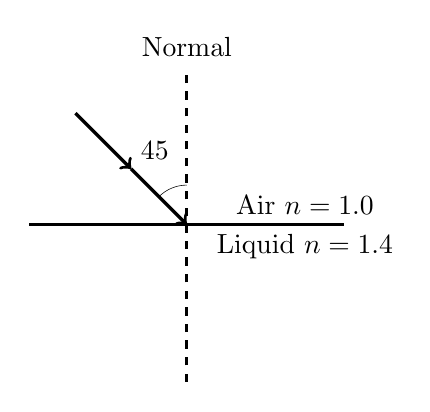
\begin{tikzpicture}
        \draw[very thick] (-2,0) -- (2,0);
        \draw[very thick,dashed] (0,-2) -- (0,2)
            node[anchor=south] {Normal};
        \draw[very thick,->] (135:2) -- (135:1);
        \draw[very thick,->] (135:1) -- (135:0);
        \node[anchor=south west] at (135:1.0) {\ang{45}};
        \draw[very thin] (135:0.5) arc (135:90:0.5);
        \node[anchor=south] at (1.5,0) {Air $n=\num{1.0}$};
        \node[anchor=north] at (1.5,0) {Liquid $n=\num{1.4}$};
    \end{tikzpicture}
    \end{center}
    \begin{choices}
        \wrongchoice{travel straight through with no bending.}
      \correctchoice{be bent toward the normal.}
        \wrongchoice{be bent away from the normal.}
        \wrongchoice{travel down the normal.}
    \end{choices}
\end{question}
}

\element{cpo-mc}{
\begin{question}{cpo-ch23-q20}
    The diagram best illustrates:
    \begin{choices}
        \wrongchoice{scattering and diffusion.}
        \wrongchoice{reflecting and interference.}
        \wrongchoice{transmission and Doppler effect.}
      \correctchoice{refraction and dispersion.}
    \end{choices}
\end{question}
}

%\element{cpo-mc}{
%\begin{question}{cpo-ch23-q21}
%    \begin{center}
%        %% NOTE: add diagram
%    \end{center}
%    The diagram shows a beam of light passing through a curved glass fiber.
%    This is possible due to the effect of:
%    \begin{choices}
%        \wrongchoice{dispersion.}
%      \correctchoice{total internal reflection.}
%        \wrongchoice{polarization.}
%        \wrongchoice{diffraction.}
%    \end{choices}
%\end{question}
%}

\element{cpo-mc}{
\begin{question}{cpo-ch23-q22}
    The color of light that is refracted most when it passes through a prism is:
    \begin{multicols}{2}
    \begin{choices}
        \wrongchoice{red}
        \wrongchoice{orange}
        \wrongchoice{green}
      \correctchoice{blue}
    \end{choices}
    \end{multicols}
\end{question}
}

%\element{cpo-mc}{
%\begin{question}{cpo-ch23-q23}
%    Which diagram correctly illustrates light rays as they pass
%        through a converging lens?
%    \begin{multicols}{2}
%    \begin{choices}
%        \wrongchoice{
%            \begin{tikzpicture}
%            \end{tikzpicture}
%        }
%    \end{choices}
%    \end{multicols}
%\end{question}
%}

\element{cpo-mc}{
\begin{question}{cpo-ch23-q24}
    The color of light for which the index of refraction is greatest is:
    \begin{multicols}{2}
    \begin{choices}
      \correctchoice{blue}
        \wrongchoice{green}
        \wrongchoice{yellow}
        \wrongchoice{red}
    \end{choices}
    \end{multicols}
\end{question}
}

\element{cpo-mc}{
\begin{question}{cpo-ch23-q25}
    The table below lists the index of refraction for various materials.
    \begin{center}
    \begin{tabular}{ll}
        \toprule
        Material    & Index of Refraction \\
        \midrule
        Vacuum  & 1.0   \\
        Air     & 1.0001 \\
        Water   & 1.33  \\
        Ice     & 1.31  \\
        Glass   & 1.5   \\
        Diamond & 2.42  \\
        \bottomrule
    \end{tabular}
    \end{center}
    As light travels from a vacuum into a substance,
        in which substance will the light experience the greatest change in direction?
    \begin{multicols}{2}
    \begin{choices}
        \wrongchoice{Air}
        \wrongchoice{Water}
        \wrongchoice{Glass}
      \correctchoice{Diamond}
    \end{choices}
    \end{multicols}
\end{question}
}

%\element{cpo-mc}{
%\begin{question}{cpo-ch23-q26}
%    The diagram below shows a ray of light ($R$) incident upon
%        a surface at an angle which is greater than the critical angle.
%    \begin{center}
%        %% NOTE: add diagram
%    \end{center}
%    Through which piont is the ray most likely to pass?
%    %% Refer to tablle 23-1A
%    \begin{multicols}{2}
%    \begin{choices}
%        \wrongchoice{$A$}
%        \wrongchoice{$B$}
%        \wrongchoice{$C$}
%      \correctchoice{$D$}
%    \end{choices}
%    \end{multicols}
%\end{question}
%}

%\element{cpo-mc}{
%\begin{question}{cpo-ch23-q27}
%    The illustration shows the image of four fish in a pond:
%    \begin{center}
%        %% NOTE: add diagram
%    \end{center}
%    If a fish is actually located at position $B$, at which position
%        would the \emph{image} of that fish appear for a person
%        looking into the pond while standing on the side of the pond?
%    %% Refer to tablle 23-1A
%    \begin{multicols}{2}
%    \begin{choices}
%      \correctchoice{$A$}
%        \wrongchoice{$B$}
%        \wrongchoice{$C$}
%        \wrongchoice{$D$}
%    \end{choices}
%    \end{multicols}
%\end{question}
%}

\element{cpo-mc}{
\begin{question}{cpo-ch23-q28}
    A light ray passes from air into a glass block.
    %%Referring to Table 23-1A
    \begin{center}
        %% NOTE: add diagram
    \end{center}
    Through which point is the ray most likely to pass?
    \begin{multicols}{2}
    \begin{choices}
        \wrongchoice{$A$}
        \wrongchoice{$B$}
      \correctchoice{$C$}
        \wrongchoice{$D$}
    \end{choices}
    \end{multicols}
\end{question}
}

%\element{cpo-mc}{
%\begin{question}{cpo-ch23-q29}
%    The diagram below represents a ray of green light passing
%        through a glas prism ($n=\num{1.61}$).
%    \begin{center}
%        %% NOTE: add diagram
%    \end{center}
%    If the same light were to pass through a prism made of
%        diamond ($n=\num{2.42}$), the path of the light
%        would be best represented by:
%    \begin{multicols}{2}
%    \begin{choices}
%        \wrongchoice{
%            \begin{tikzpicture}
%            \end{tikzpicture}
%        }
%    \end{choices}
%    \end{multicols}
%\end{question}
%}

\element{cpo-mc}{
\begin{question}{cpo-ch23-q30}
    A light ray passes through a converging lens, but does not bend.
    Describe its path.
    \begin{choices}
        \wrongchoice{Above the optical axis.}
        \wrongchoice{Below the optical axis.}
      \correctchoice{Along the optical axis.}
        \wrongchoice{Crossing the optical axis.}
    \end{choices}
\end{question}
}

%% NOTE: both positive and negative film exist
%\element{cpo-mc}{
%\begin{question}{cpo-ch23-q31}
%    When photographic film is exposed to light,
%        the image produced on film is called a:
%    \begin{choices}
%        \wrongchoice{positive.}
%      \correctchoice{negative.}
%        \wrongchoice{CCD.}
%        \wrongchoice{pixel.}
%    \end{choices}
%\end{question}
%}

\element{cpo-mc}{
\begin{question}{cpo-ch23-q32}
    Lenses that are thicker around the edges of the lens than in the middle are:
    \begin{multicols}{2}
    \begin{choices}
        \wrongchoice{convex}
        \wrongchoice{converging}
      \correctchoice{diverging}
        \wrongchoice{dividing}
    \end{choices}
    \end{multicols}
\end{question}
}

\element{cpo-mc}{
\begin{question}{cpo-ch23-q33}
    All of the following statements about images are correct \emph{except} that images:
    \begin{choices}
        \wrongchoice{are organized light}
      \correctchoice{can be touched like any object}
        \wrongchoice{can be formed by lenses}
        \wrongchoice{form where light rays converge}
    \end{choices}
\end{question}
}

\element{cpo-mc}{
\begin{question}{cpo-ch23-q34}
    The type of image that can be projected on a screen is always:
    \begin{multicols}{2}
    \begin{choices}
        \wrongchoice{virtual}
      \correctchoice{real}
        \wrongchoice{enlarged}
        \wrongchoice{smaller}
    \end{choices}
    \end{multicols}
\end{question}
}

\element{cpo-mc}{
\begin{question}{cpo-ch23-q35}
    A lens is used to produce an image of an object.
    If the object is \SI{4}{\centi\meter} tall and the image is \SI{12}{\centi\meter} high,
        the magnification of that lens is:
    \begin{multicols}{4}
    \begin{choices}
        \wrongchoice{48}
        \wrongchoice{16}
        \wrongchoice{8}
      \correctchoice{3}
    \end{choices}
    \end{multicols}
\end{question}
}

\element{cpo-mc}{
\begin{question}{cpo-ch23-q36}
    A virtual image of an object will be produced by a converging lens if the object is placed:
    \begin{choices}
        \wrongchoice{more than five focal lengths from the lens.}
        \wrongchoice{precisely two focal lengths from the lens.}
        \wrongchoice{just beyond one focal length from the lens.}
      \correctchoice{closer to the lens that one focal length.}
    \end{choices}
\end{question}
}

%\element{cpo-mc}{
%\begin{question}{cpo-ch23-q37}
%    In the diagram below, $f$ represents the focal point
%        and $2f$ represents a point at twice the focal length from the lens.
%    \begin{center}
%    \begin{tikzpicture}
%        %% NOTE: TODO: draw tikz
%    \end{tikzpicture}
%    \end{center}
%    In which direction does most of the light in ray $R$ pass?
%    \begin{multicols}{4}
%    \begin{choices}
%        \wrongchoice{$A$}
%      \correctchoice{$B$}
%        \wrongchoice{$C$}
%        \wrongchoice{$D$}
%    \end{choices}
%    \end{multicols}
%\end{question}
%}

%% NOTE: \frac{1}{f} = \frac{n-n_0}{n_0} \left(\frac{1}{R_1}-\frac{1}{R_2}\right)

%\element{cpo-mc}{
%\begin{question}{cpo-ch23-q38}
%    In the diagram below, $f$ represents the focal point
%        and $2f$ represents a point at twice the focal length from the lens.
%    Which ray diagram best represents the formation of a real,
%        enlarged image of the object?
%    \begin{multicols}{2}
%    \begin{choices}
%        %% NOTE: TODO: draw tikz
%        \wrongchoice{
%            \begin{tikzpicture}
%            \end{tikzpicture}
%        }
%    \end{choices}
%    \end{multicols}
%\end{question}
%}

%\element{cpo-mc}{
%\begin{question}{cpo-ch23-q39}
%    In the diagram below, $f$ represents the focal point
%        and $2f$ represents a point at twice the focal length from the lens.
%    Which ray diagram best represents the formation of a virtual,
%        reduced image of the object?
%    \begin{multicols}{2}
%    \begin{choices}
%        %% NOTE: TODO: draw tikz
%        \wrongchoice{
%            \begin{tikzpicture}
%            \end{tikzpicture}
%        }
%    \end{choices}
%    \end{multicols}
%\end{question}
%}

\element{cpo-mc}{
\begin{question}{cpo-ch23-q40}
    The image produced by a diverging lens is always:
    \begin{choices}
        \wrongchoice{smaller and upside down}
        \wrongchoice{larger and upside down}
      \correctchoice{smaller and right-side-up}
        \wrongchoice{larger and right-side-up}
    \end{choices}
\end{question}
}

\element{cpo-mc}{
\begin{question}{cpo-ch23-q41}
    How many numbers must be stored in order to record
        a \num{3} megapixel colored image on a CCD?
    \begin{multicols}{2}
    \begin{choices}
        \wrongchoice{\num{256}}
        \wrongchoice{\num{788}}
        \wrongchoice{\num{3e6}}
      \correctchoice{\num{9e6}}
    \end{choices}
    \end{multicols}
\end{question}
}


\endinput


